\documentclass[review]{elsarticle}

\usepackage{lineno,hyperref}
\modulolinenumbers[5]
\usepackage{booktabs}
\usepackage{graphicx}
\usepackage{float}
\graphicspath{ {./images/} }



\journal{International Journal of Forecasting}

%%%%%%%%%%%%%%%%%%%%%%%
%% Elsevier bibliography styles
%%%%%%%%%%%%%%%%%%%%%%%
%% To change the style, put a % in front of the second line of the current style and
%% remove the % from the second line of the style you would like to use.
%%%%%%%%%%%%%%%%%%%%%%%

%% Numbered
%\bibliographystyle{model1-num-names}

%% Numbered without titles
%\bibliographystyle{model1a-num-names}

%% Harvard
%\bibliographystyle{model2-names.bst}\biboptions{authoryear}

%% Vancouver numbered
%\usepackage{numcompress}\bibliographystyle{model3-num-names}

%% Vancouver name/year
%\usepackage{numcompress}\bibliographystyle{model4-names}\biboptions{authoryear}

%% APA style
%\bibliographystyle{model5-names}\biboptions{authoryear}

%% AMA style
%\usepackage{numcompress}\bibliographystyle{model6-num-names}

%% `Elsevier LaTeX' style
\bibliographystyle{elsarticle-num}
%%%%%%%%%%%%%%%%%%%%%%%

\begin{document}

\begin{frontmatter}

\title{A novel electricity probabilistic price forecasting using deep residual neural networks for GEFCOm2014}
\tnotetext[mytitlenote]{Fully documented templates are available in the elsarticle package on \href{http://www.ctan.org/tex-archive/macros/latex/contrib/elsarticle}{CTAN}.}

%% Group authors per affiliation:
% \author{Pornchai Chaweewat\fnref{myfootnote}}
\author{Pornchai Chaweewat\fnref{myfootnote}}

\address{AIT}
% \fntext[myfootnote]{Since 1880.}

% %% or include affiliations in footnotes:
% \author[mymainaddress,mysecondaryaddress]{Elsevier Inc}
% \ead[url]{www.elsevier.com}
%
% \author[mysecondaryaddress]{Global Customer Service\corref{mycorrespondingauthor}}
% \cortext[mycorrespondingauthor]{Corresponding author}
% \ead{support@elsevier.com}
%
% \address[mymainaddress]{1600 John F Kennedy Boulevard, Philadelphia}
% \address[mysecondaryaddress]{360 Park Avenue South, New York}

\begin{abstract}
What we do? - This paper proposes a electricity price forecasting approach based on a novel residual neural network for probabilistic electricity price forecasting under price spike environment for GEFCom2014.

Why I do this? - The electricity price, in deregulation electricity market, has become more fluctuated and generally unanticipated price spike. The use of prediction interval or probabilistic forecasting has become much more common due to it help market participants to submit effective bid with low risks.

How I do this? - A new model is developed from novel deep residual neural network approach. It consists of two major part. First is spike prediction. Interval's value forecasting is another which is formulated into two methods; upper-lower bounds and mean-variance method. The proposed methodology is test with GEFCom2014 dataset where there are 15 tasks for electricity price forecasting which high and spike price are include.
The novel method is tested with non-price spike electricity price foreasting model as benchmark.

What is the result? - The overall results show that the proposed method with confidence levels at 90$\%$ and 80$\%$ can imporve reliability and narrow width of prediction interval under non and high number of high and spike price tasks. The model can handle in spike price occurances environment where it is realistic globally.

\end{abstract}

\begin{keyword}
Residual neural network, GEFCom2014
\end{keyword}

\end{frontmatter}

\linenumbers

\section{Introduction}

  Since the transformation of the deregulation of modern power systems, electricty price forecasting has become more important process to energy market's participants at planning and operation levels. The electricity price in deregulation has become more and more fluctuated as well as the number of the price spikes occurence has been increasing. The occurrence of price spikes can cause financial damage to both customers and producers. Price spike can be several times to thousand times of the normal price. Price spike appears due to Increasing intermittent electricity production makes electricity prices more volatile, with spikes appearing either as very high prices (due to sudden lack of available generation) or as negative prices (due to excess of renewable generation). Several evidences shows that the price spike around 100$\$$/MWhr may simply resulted from normal congestion or unexpected overload, while price spike around $\$$500/MWhr led by lacking of reserve. This case the day ahead clearing price is the dominant feature what indicate insufficient reserve. The price spike above $\$$1,000/MWhr should be the consequence of the outage or breakdown of the generation or transmission system. Such outage or breakdown many comes from many factors, like weather, load profile, etc  \cite{He2016}. \cite{SINGHAL2011550} provide fundamental reasons of price spike which are volatility of fuel price, load uncertainty, fluctuation in hydroelectricity production, generation outage, transmission congestion, behavior of market participation and market manipulation. \cite{GONZALEZSOTRES2017338} studied on technique and economical of on centralized voltage control with high PV penetration in Portuguese network. The results show that improvement in both forecasting tools and communication systems have significant impact on dedicate resources and voltage control.



  (talk about point of forecating, 1 method, 2 measurement, 3 problems) Over the past few decades, many powerful forecasting algorithms have been developed (for a recent comprehensive review, see \cite{Weron2014}). The majority of emprical studies are on point forecasting (or call expected value of the spot price).

  (mention about problems of poing of forecasting, introduct to interval forecasting)

  (mention on used of deep residual neural network and why we use this method)
  Deep residual network is modified from deep Feed Forward Neural Networks (FFNNs) with extra connections (or called skip connections), passing input from one layer to a late layer as well as the next layer as shown in figure~\ref{Fig:Basic_DRN}. DRN is widely used in computer vision and pattern reconigtion. There are few used on deep residual neural network.

  \begin{figure}[H]
    \caption{Basis DRN}
    \label{Fig:Basic_DRN}
    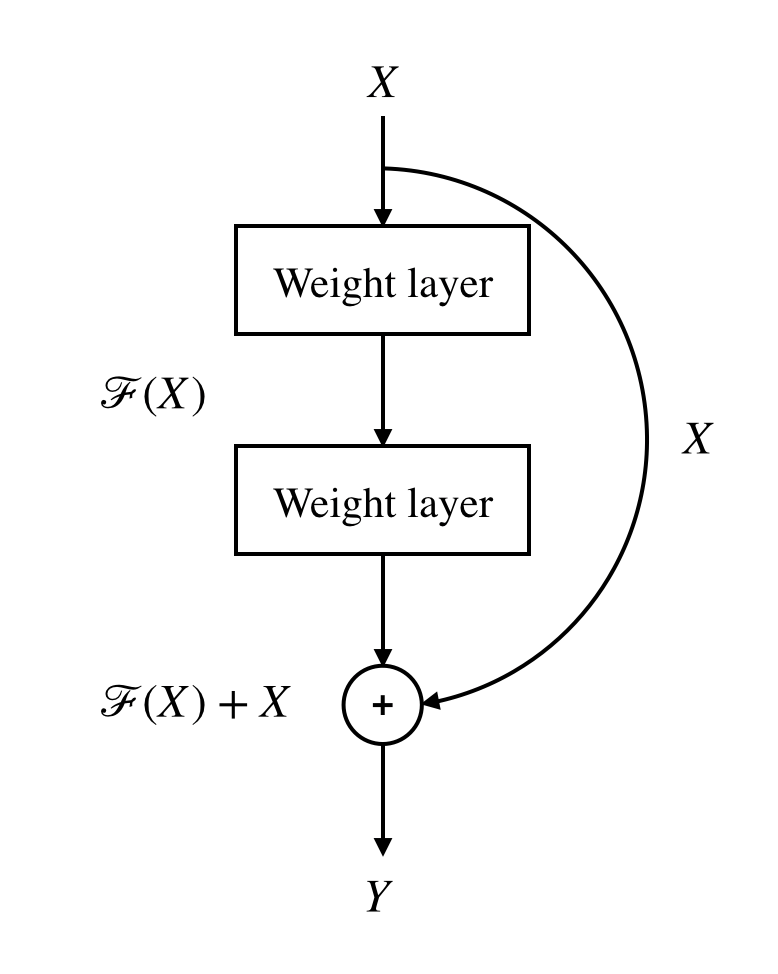
\includegraphics[width=5cm]{basic_DRN}
  \centering
  \end{figure}


  (proposeal) Therefore, this paper seeks to apply

  (structure) The remainder of the paper is organized as follows. First, the problem formulation is presented in brief in section 2. The, the main features of the ANN algorithm are presented in section 3. Next, the results after prediction in different cases of proposed method  are discussed in section 4. Finally, conclusions are drawn in the last section of this paper.

\section{Problem formulation}

  \subsection{Interval forecasting}

  \subsection{Measurement}
    The performance of the proposed model need to be assessed in term of the quaility of of prediction interval, namely converage probability and PI width. First,  PI converage probility (PICP) refers to the ability of the constructed PIs to capture the actual target variables. PICP can be methematically stated as

    \begin{equation}
      PICP = \frac{1}{N} \sum_{i=1}^{N} C_{i}
      \label{eq.PICP}
    \end{equation}

    where

    \begin{equation}
      C_{i} =
      \begin{cases}
        1, if t_{i} \in [L_{i},U_{i}] \\
        0, if t_{i} \not\in [L_{i},U_{i}]
      \end{cases}
      \label{eq.Ci}
    \end{equation}

    where $N$ is the number of samples in the test set, $t_{i}$ represents the actual target, and $L_{i}$ and $U_{i}$ are lower and upper bounds of hte $i$th PI, repestively. The range of PICP lies between 0$\%$ (wher none of hte targets are enclosed by PI) to 100$\%$ (when all targets are enclosed by PI). Ideally, PICP should be very close or larger than the norminal confidence level associated to the PIs.
    PICP has a direct relationship with the width of PIs. A satisfactorily large PICP can be easily achieved by widening PIs from either side. However, such PIs are too conservative and less useful in practice, as they do not show the variation of the targetes. Therefore, a measure is resquired to check how wide the PIs are. Mean PI Width (MPIW) quantifies this aspect of PIs \cite{Khosravi2010}.

    \begin{equation}
      MPIW = \frac{1}{N} \sum_{i=1}^{N} (U_{i}-L_{i})
      \label{eq.MPIW}
    \end{equation}

    Secondrly, MPIW shows the average width of PIs. Normalizing MPIW by the range of the underlying target, $R$, allows us to compare PIs constructed for different datasets repectively (the new measure is called NMPIW),
    \begin{equation}
      NMPIW = \frac{NMPIW}{R}
      \label{eq.NMPIW}
    \end{equation}

    Both PICP and NMPIW, are representing quality and width of PIs, evaluate the quality of PIS from one aspect. A combined index is required for the comprehensive assessment of PIs from both coverage probility and width perspectives. The new measure should give a higher priority to PICP, as it is the key feature of PIs determining whether constructed PIs are theoretically correcty or not. The Coverage Width-baed Criterion (CWC) evalutes PIs from both coverage probility and width perspectives.

    Where, $\eta$ and $\mu$ are two hyperparameters controlling the location and amount of CWC jump. These measures can be easily determined based on the level of confidence associated with PIs. $\mu$ correspomds to the nominal confidence level associated with PIs and can be set to 1-$\alpha$. The design of CWC is based on two principles:

    \begin{itemize}
      \item if PICP is less than the nominal confidence level, (1-$\alpha$)$\%$, CWC should be large regardless of the width of PIs (measures by NMIPW),
      \item if PICP is greater than or equal to its corresponding confidence level, then NMPIW should be the influential factor. $\gamma$(PICP), eliminates the exponential term of CWC when PICP is greater or equal to the nominal confidence level.
    \end{itemize}

  \subsection{Data description}
    All data in this paper is provided in Global Energy Forecasting Competition 2014 (see \cite{Hong2016}). The aim of this competition is to forecast 15 tasks of electricity prices in term of probabilistic distribution (in quantiles). Hourly data of locational marginal price (LMP), zonal load forecast and system load forecast are provided. The participants receive historical data and forecast for next day electricty price. In total, the price forecasting track involves about three years of locational marginal price, zonal and system load forecast. The summarized solution data set of 15 tasks is shown in table~\ref{table:price_data_set}.

    \begin{table}[htbp]
      \caption{GEFcom2014 task solution}
      \begin{center}
      \begin{tabular}{|c|c|c|c|c|c|c|}
      \hline
      Task & Day & Holiday & Season & Normal price & High price & Spike price\\
      \hline
      1 & Sun & Yes & Summer & 24 & - & -\\
      2 & Mon & No & Summer & 24 & - & -\\
      3 & Mon & No & Summer & 22 & 2 & -\\
      4 & Thu & No & Summer & 24 & - & -\\
      5 & Tue & No & Summer & 22 & 2 & -\\
      6 & Sat & Yes & Summer & 24 & - & -\\
      7 & Tue & No & Summer & 16 & 8 & -\\
      8 & Thu & No & Summer & 12 & 8 & 4\\
      9 & Fri & No & Summer & 13 & 6 & 5\\
      10 & Sat & Yes & Summer & 18 & 6 & -\\
      11 & Wed & No & Summer & 24 & - & -\\
      12 & Thu & No & Summer & 24 & - & -\\
      13 & Sat & Yes & Authumn & 24 & - & -\\
      14 & Sun & Yes & Authumn & 24 & - & -\\
      15 & Tue & No & Authumn & 15 & 9 & -\\
      \hline
      \end{tabular}
      \label{table:price_data_set}
      \end{center}
    \end{table}


    The participation teams in GEFCom2014 perform electricity price forecasting method i.e.; linear regression (IR)\cite{Dudek2016}, multilayer perceptron (MLP)\cite{Dudek2016},  multiple quantile regression\cite{Juban2016}, hybrid quantile estimation with pre-and-post processes\cite{Maciejowska2016}.
    % Where, table~\ref{table:GEFCOm2014} summarizes top four team's method.
    % \begin{table}[H]
    %   \caption{Summary of the methods used by the top four teams of the price forecasting track. Techniques}
    %   \label{table:GEFCOm2014}
    %   \begin{tabular}{p{2cm}p{5cm}p{3cm}p{3cm}}
    %   \hline
    %                          & Techniques                                                                                                                                                                  & Spike preprocessing                                                                                     & Forecast combination \\ \hline
    %   Tololo                 & (1) Quantile regression, generalized additive models; (2) autoregressive models, random forest regression, gradient boosting machine; (3) Kernel based quantile regression. & Preprocessed spikes for some of the models.                                                             & ML-Poly aggregation  \\
    %   Team Poland            & Autoregressive models with exogenous variables; filtering; quantile regression; judgmental forecasting                                                                      & Three filtering methods: day type filtering, similar load profile filtering and expected bias filtering & Arithmetic average   \\
    %   GMD                    & Feed forward neural network                                                                                                                                                 & None                                                                                                    & None                 \\
    %   C3 Green Team          & Quantile regression; radial basis function network; k-means algorithm; alternating direction method of multipliers; Autoregressive models with exogenous variables          & None                                                                                                    & None                 \\ \hline
    %   \end{tabular}
    %
    % \end{table}

\section{Proposed probabilisitic deep residual neural network}
  As mention eariler,

  \begin{figure}[H]
    \caption{Upper and lower bound and mean and variance estimation}
    \label{Fig:UB_LB_MV_PDRN}
    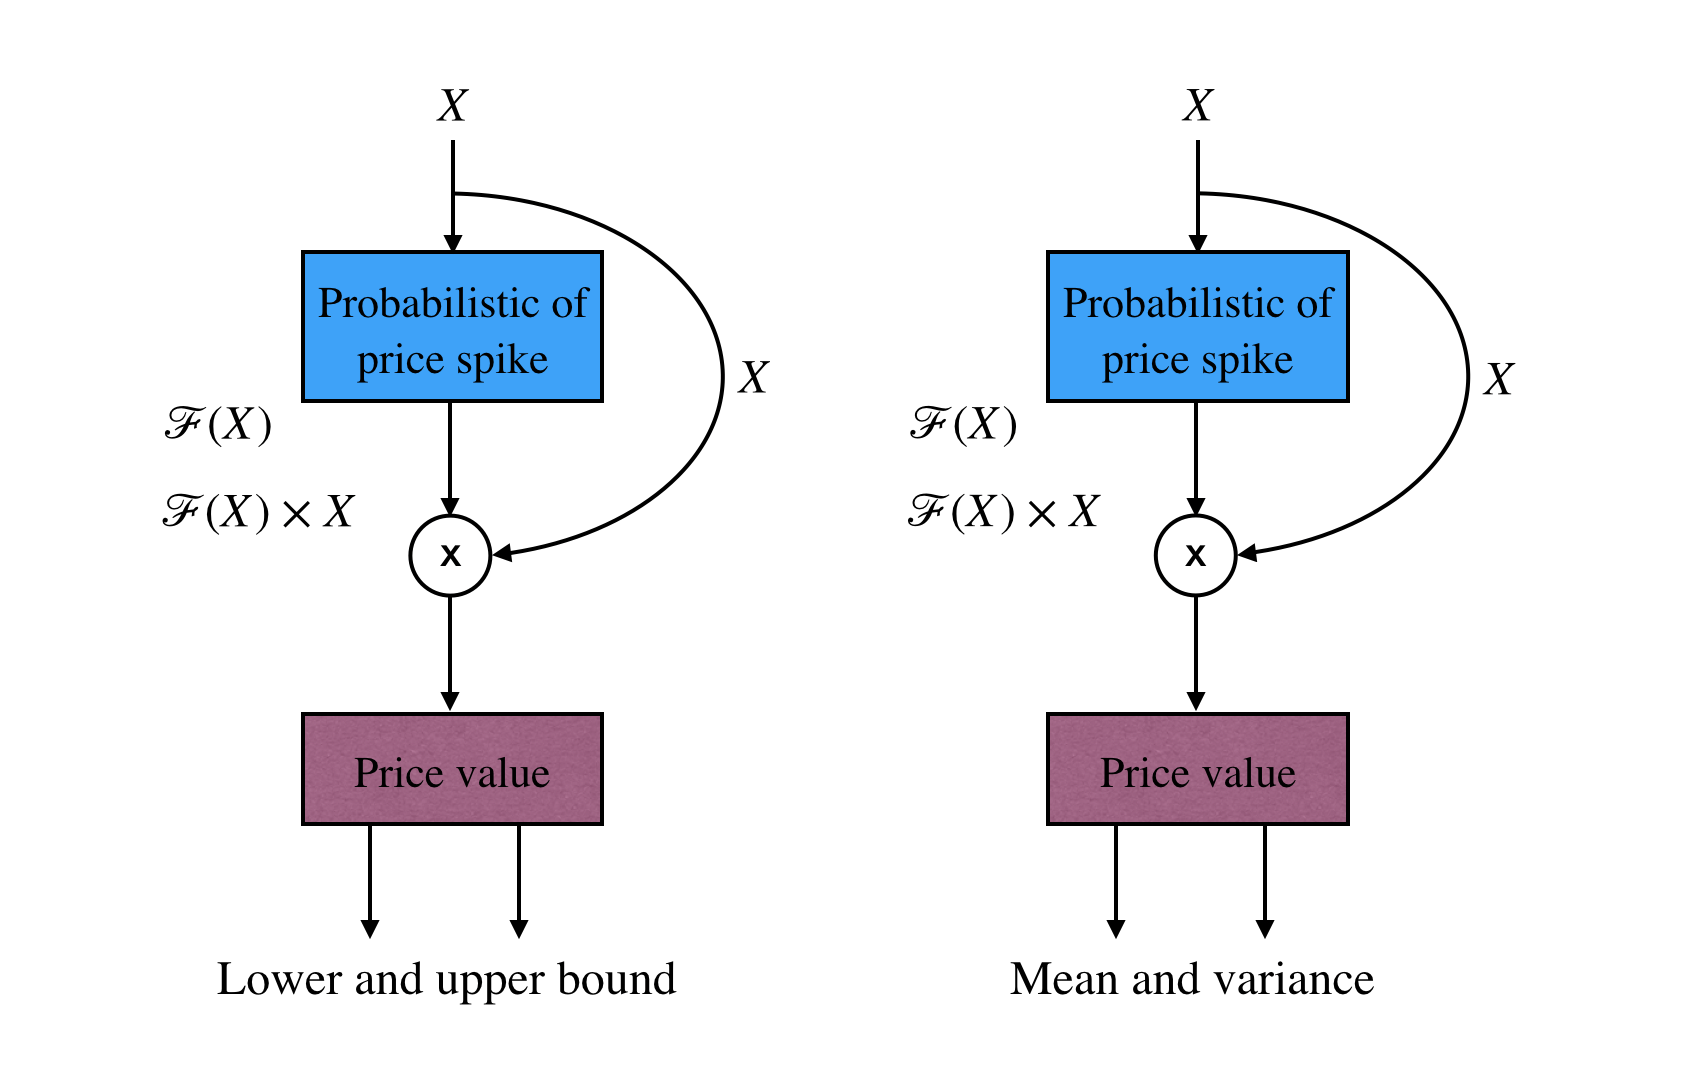
\includegraphics[width=12cm]{UB_LB_MV_PDRN}
  \centering
  \end{figure}

  \begin{figure}[H]
    \caption{Proposed probabilistic deep residual network}
    \label{Fig:proposed_PDRN}
    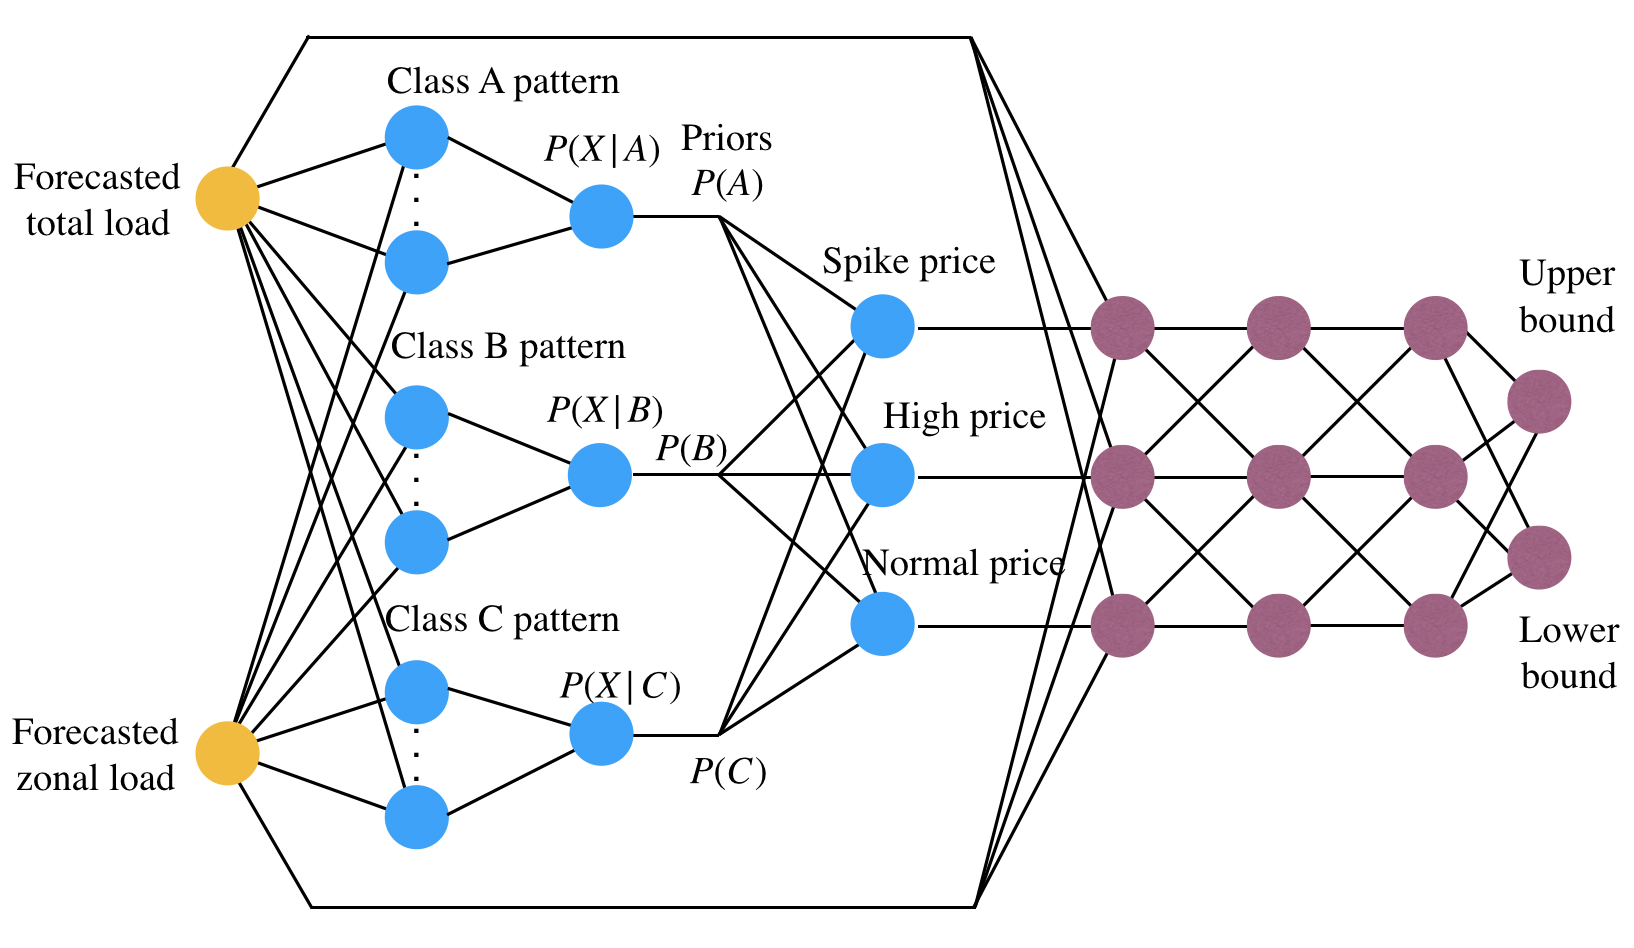
\includegraphics[width=12cm]{proposed_PDRN}
  \centering
  \end{figure}


\section{Conclusions}
This paper proposes a novel application of residual neural network based approach to probabilistic electricity price forecasting.

% \section{The Elsevier article class}
%
% \paragraph{Installation} If the document class \emph{elsarticle} is not available on your computer, you can download and install the system package \emph{texlive-publishers} (Linux) or install the \LaTeX\ package \emph{elsarticle} using the package manager of your \TeX\ installation, which is typically \TeX\ Live or Mik\TeX.
%
% \paragraph{Usage} Once the package is properly installed, you can use the document class \emph{elsarticle} to create a manuscript. Please make sure that your manuscript follows the guidelines in the Guide for Authors of the relevant journal. It is not necessary to typeset your manuscript in exactly the same way as an article, unless you are submitting to a camera-ready copy (CRC) journal.
%
% \paragraph{Functionality} The Elsevier article class is based on the standard article class and supports almost all of the functionality of that class. In addition, it features commands and options to format the
% \begin{itemize}
% \item document style
% \item baselineskip
% \item front matter
% \item keywords and MSC codes
% \item theorems, definitions and proofs
% \item lables of enumerations
% \item citation style and labeling.
% \end{itemize}
%
% \section{Front matter}
%
% The author names and affiliations could be formatted in two ways:
% \begin{enumerate}[(1)]
% \item Group the authors per affiliation.
% \item Use footnotes to indicate the affiliations.
% \end{enumerate}
% See the front matter of this document for examples. You are recommended to conform your choice to the journal you are submitting to.
%
% \section{Bibliography styles}
%
% There are various bibliography styles available. You can select the style of your choice in the preamble of this document. These styles are Elsevier styles based on standard styles like Harvard and Vancouver. Please use Bib\TeX\ to generate your bibliography and include DOIs whenever available.
%
% Here are two sample references: .

\section*{References}

\bibliography{mybibfile}

\end{document}
